\documentclass[a4paper, 12pt]{article}
\usepackage{geometry}
\geometry{verbose,a4paper,tmargin=2cm,bmargin=2cm,lmargin=2cm,rmargin=2cm}
\usepackage{fontspec}
\setmainfont[
  Ligatures=TeX,
  Extension=.otf,
  UprightFont=*-regular,
  ItalicFont=*-italic,
  BoldFont=*-bold,
  BoldItalicFont=*-bolditalic,
]{xits}
\usepackage[english,russian]{babel}

\newif\ifisinsp
\newif\ifisone
\newif\ifisname
\newif\ifisnum
\isinsptrue
\isonetrue
\isnamefalse
\isnumtrue

\def \labtype {Лабораторная}
% Это для нумерации страниц после титульника
\usepackage{fancyhdr}
\pagestyle{fancy}
\renewcommand{\headrulewidth}{0pt}
\fancyfoot[C] {\thepage}

\isnametrue
\def \labnum {1}
\def \labsubj {Методы обработки цифровых сигналов}
\def \labauthor {Чебыкин И. Б.}
\def \labgroup {P3401}
\def \labinsp {Тропченко А. А.}
\def \labname {Вариант 12}

\usepackage{graphicx,tabularx}

\usepackage{caption}
\usepackage{verbatim}
\usepackage[dvipsnames]{xcolor}

\usepackage{fancyvrb}

\RecustomVerbatimCommand{\VerbatimInput}{VerbatimInput} {
 fontsize=\scriptsize,
 %
 frame=lines,  % top and bottom rule only
 framesep=2em, % separation between frame and text
 rulecolor=\color{Gray},
 %
 label=\fbox{\color{Black}source},
 labelposition=topline,
 %
}

\captionsetup{labelsep=period}
\pagestyle{fancy}
\begin{document}
\begin{titlepage}
	\begin{center}
		\large
		Университет ИТМО

		\vspace{0.25cm}
		
		Факультет программной инженерии и компьютерной техники
		
		Кафедра вычислительной техники
		\vfill
		
		\textsc{\labtype\spaceработа \ifisnum № \labnum{} \fi по дисциплине \\"\labsubj" \ifisname\small \\ \labname \fi}
			
		\bigskip
	\end{center}
	\vfill
	\vfill
	
	\begin{flushright}
	\ifisone
	Выполнил: \labauthor
	\else
	Выполнили: \labauthor
	\fi

	\vspace{0.25cm}
	Группа: \labgroup
			
	\vspace{0.25cm}
	\ifisinsp
	Проверяющий: \labinsp
	\fi
	\end{flushright}
	\vfill
	
	\begin{center}
	СПб, \the\year
	\end{center}
\end{titlepage}

\section{Цель работы}
Цель работы - определение возможностей метода когерентного накопления
для случаев стационарного и квазистационарного сигнала.
\section{Задание}

Вид сигнала: сумма двух гармонических

Соотношение сигнал/шум: 0.4

Число циклов накопления: до 1000

Пределы изменения соотношения сигнал/шум: 0.2 - 3

\section{Стационарный сигнал}
\subsection{Зависимость SNR от числа накоплений}
\begin{tabular}{|c|c|}
\hline
M & $SNR_{out}$\\ \hline
10 & 3.868\\ \hline
25 & 5.5653\\ \hline
50 & 9.211\\ \hline
75 & 9.6655\\ \hline
100 & 10.6286\\ \hline
125 & 12.3413\\ \hline
150 & 11.7916\\ \hline
200 & 14.9548\\ \hline
250 & 15.2979\\ \hline
300 & 16.1758\\ \hline
350 & 17.383\\ \hline
400 & 17.1882\\ \hline
450 & 17.2875\\ \hline
500 & 16.8379\\ \hline
550 & 17.6479\\ \hline
600 & 17.19\\ \hline
650 & 16.087\\ \hline
700 & 17.9941\\ \hline
750 & 16.107\\ \hline
800 & 14.964\\ \hline
850 & 15.4224\\ \hline
900 & 15.6997\\ \hline
950 & 14.021\\ \hline
1000 & 14.4387\\ \hline
\end{tabular}

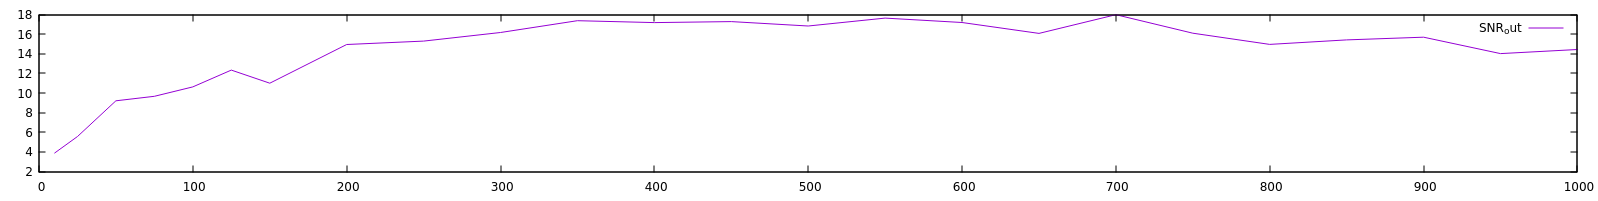
\includegraphics[width=\textwidth]{img/r1.png}

\subsection{Зависимость $SNR_{out}$ от $SNR_{in}$}

\begin{tabular}{|c|c|}
\hline
$SNR_{in}$ & $SNR_{out}$\\ \hline
0.2 & 2.1394\\ \hline
0.5 & 5.1397\\ \hline
0.8 & 7.9533\\ \hline
1.0 & 9.2874\\ \hline
1.3 & 10.6212\\ \hline
1.6 & 12.3531\\ \hline
1.9 & 15.134\\ \hline
2.2 & 17.0636\\ \hline
2.5 & 18.9606\\ \hline
2.8 & 19.696\\ \hline
3.0 & 20.9596\\ \hline
\end{tabular}
\begin{tabular}{|c|c|}
\hline
$SNR_{in}$ & $SNR_{out}$\\ \hline
0.2 & 3.9808\\ \hline
0.5 & 7.1364\\ \hline
0.8 & 10.2323\\ \hline
1.0 & 12.8602\\ \hline
1.3 & 14.8341\\ \hline
1.6 & 19.6691\\ \hline
1.9 & 18.976\\ \hline
2.2 & 21.0165\\ \hline
2.5 & 23.8579\\ \hline
2.8 & 24.7976\\ \hline
3.0 & 25.7825\\ \hline
\end{tabular}
\begin{tabular}{|c|c|}
\hline
$SNR_{in}$ & $SNR_{out}$\\ \hline
0.2 & 3.9808\\ \hline
0.5 & 11.1466\\ \hline
0.8 & 13.6484\\ \hline
1.0 & 16.5936\\ \hline
1.3 & 18.889\\ \hline
1.6 & 23.2473\\ \hline
1.9 & 24.3314\\ \hline
2.2 & 24.9963\\ \hline
2.5 & 26.9554\\ \hline
2.8 & 27.951\\ \hline
3.0 & 29.7736\\ \hline
\end{tabular}

\vspace*{100bp}


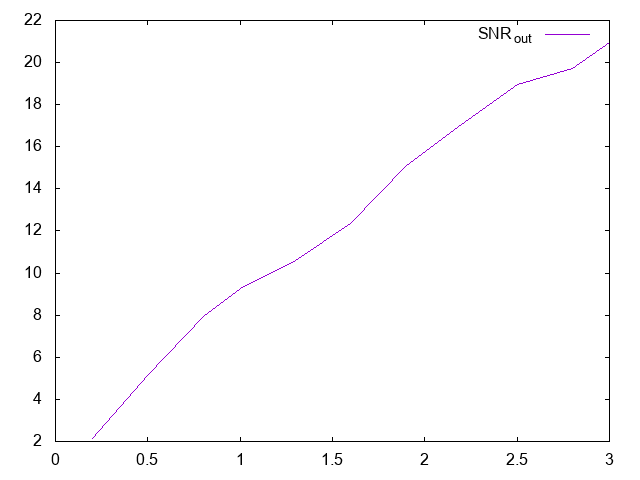
\includegraphics[scale=0.7,natwidth=320bp,natheight=240bp]{img/output_r22m10.csv.png}

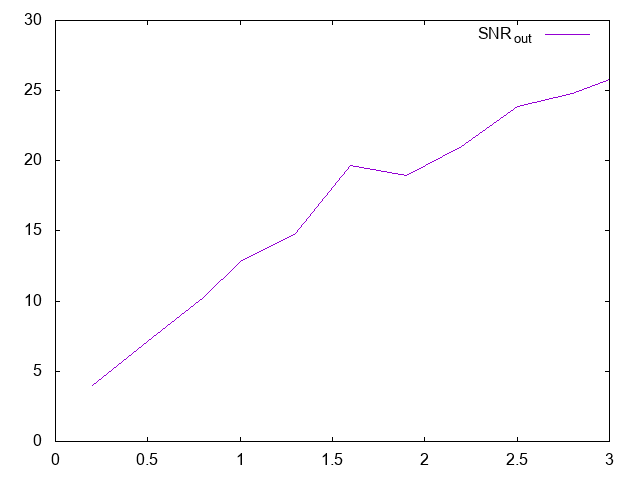
\includegraphics[scale=0.7,natwidth=320bp,natheight=240bp]{img/output_r22m25.csv.png}

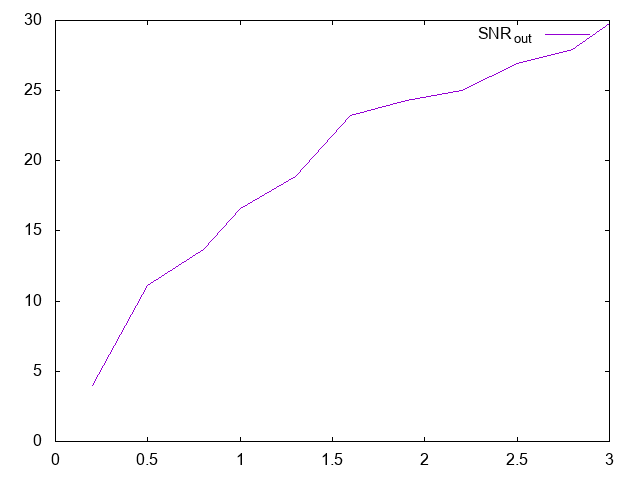
\includegraphics[scale=0.7,natwidth=320bp,natheight=240bp]{img/output_r22m50.csv.png}

\section{Квазистационарный сигнал}

\subsection{Зависимость SNR от числа накоплений}

\begin{tabular}{|c|c|}
\hline
M & $SNR_{out}$\\ \hline
10 & 2.1455\\ \hline
25 & 0.9983\\ \hline
50 & 1.0068\\ \hline
75 & 1.0065\\ \hline
100 & 1.0005\\ \hline
125 & 1.0062\\ \hline
150 & 1.0002\\ \hline
200 & 1.0004\\ \hline
300 & 0.9992\\ \hline
400 & 0.9989\\ \hline
500 & 0.9994\\ \hline
600 & 0.9997\\ \hline
700 & 0.9987\\ \hline
800 & 0.9997\\ \hline
900 & 1.0003\\ \hline
1000 & 0.9997\\ \hline
\end{tabular}

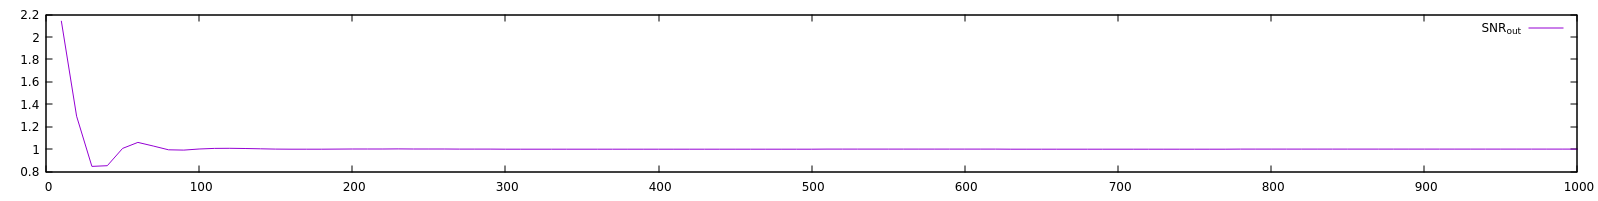
\includegraphics[width=\textwidth]{img/r3.png}

\subsection{Зависимость $SNR_{out}$ от $SNR_{in}$}

\begin{tabular}{|c|c|}
\hline
$SNR_{in}$ & $SNR_{out}$\\ \hline
0.1 & 1.1167\\ \hline
0.3 & 1.895\\ \hline
0.5 & 2.1124\\ \hline
0.7 & 2.2351\\ \hline
0.9 & 2.316\\ \hline
1.1 & 2.3744\\ \hline
1.5 & 2.4657\\ \hline
1.9 & 2.5114\\ \hline
2.1 & 2.5527\\ \hline
2.5 & 2.5032\\ \hline
2.9 & 2.5593\\ \hline
3.0 & 2.5621\\ \hline
\end{tabular}
\begin{tabular}{|c|c|}
\hline
$SNR_{in}$ & $SNR_{out}$\\ \hline
0.1 & 0.9149\\ \hline
0.3 & 0.9916\\ \hline
0.5 & 1.0081\\ \hline
0.7 & 1.0271\\ \hline
0.9 & 1.0138\\ \hline
1.1 & 1.0209\\ \hline
1.5 & 1.0193\\ \hline
1.9 & 1,0213\\ \hline
2.1 & 1.0229\\ \hline
2.5 & 1.0181\\ \hline
2.9 & 1.0202\\ \hline
3.0 & 1.0201\\ \hline
\end{tabular}
\begin{tabular}{|c|c|}
\hline
$SNR_{in}$ & $SNR_{out}$\\ \hline
0.1 & 0.9924\\ \hline
0.3 & 0.9956\\ \hline
0.5 & 0.992\\ \hline
0.7 & 1.0043\\ \hline
0.9 & 1.0024\\ \hline
1.1 & 0.9966\\ \hline
1.5 & 1.0017\\ \hline
1.9 & 1.0024\\ \hline
2.1 & 1.0023\\ \hline
2.5 & 1.002\\ \hline
2.9 & 0.9996\\ \hline
3.0 & 1.0006\\ \hline
\end{tabular}

\vspace*{100bp}


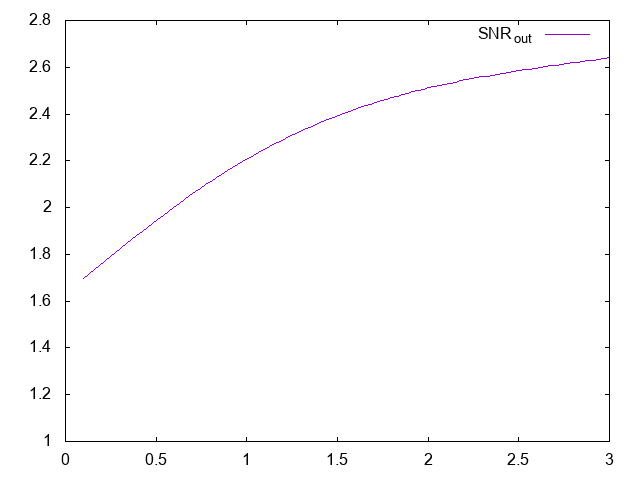
\includegraphics[scale=0.7,natwidth=320bp,natheight=240bp]{img/output_r4m10.csv.png}

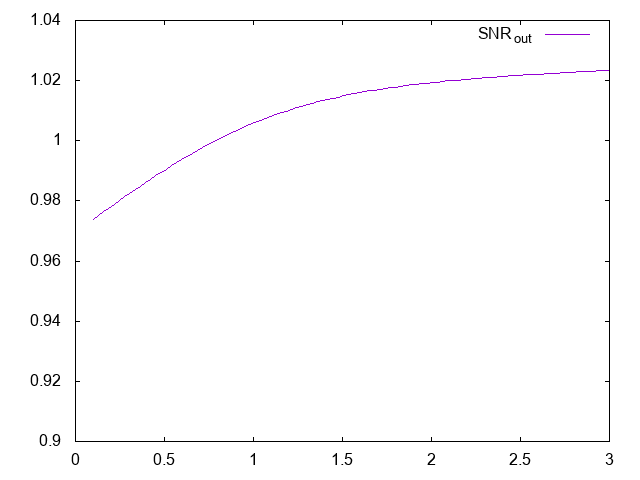
\includegraphics[scale=0.7,natwidth=320bp,natheight=240bp]{img/output_r4m25.csv.png}

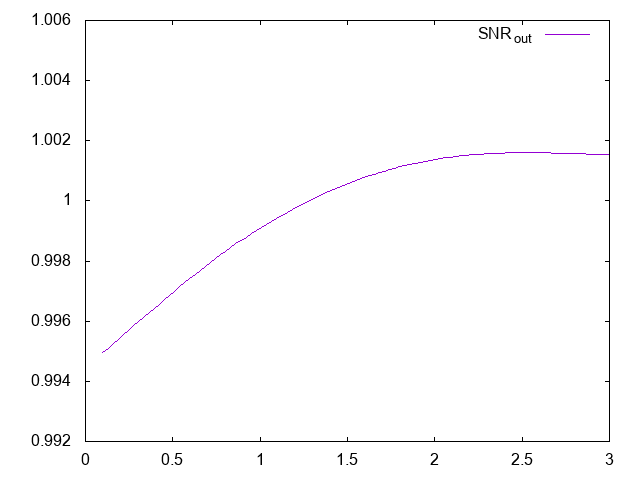
\includegraphics[scale=0.7,natwidth=320bp,natheight=240bp]{img/output_r4m50.csv.png}

\section{Функциональная схема устройства}

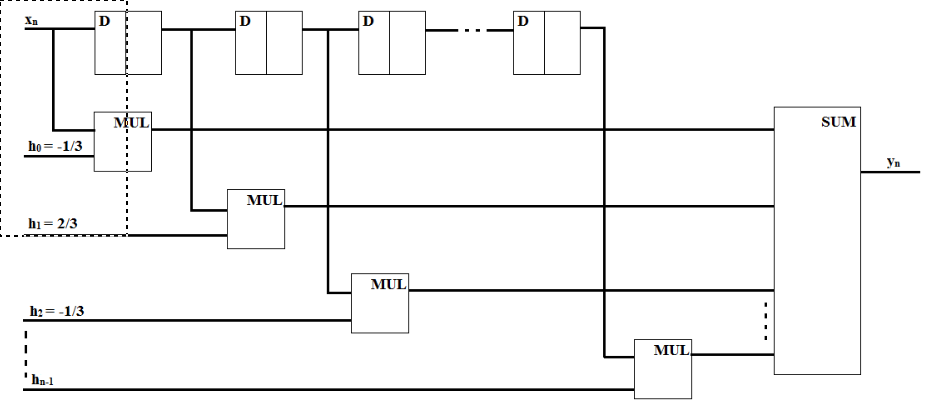
\includegraphics[scale=0.6]{img/scheme.png}

\section{Вывод}

В ходе данной лабораторной работы я ознакомился с методом когерентного накопления
для стационарного и квазистационарного сигналов. В результате подтвердилось,
что этот метод эффективен, если сигнал постоянен.


\end{document}
